\documentclass[border=6pt]{standalone}
\usepackage{tikz}
\usepackage{pgfplots}
\pgfplotsset{compat=1.18}
\usetikzlibrary{arrows.meta,positioning,shapes.geometric,fit,backgrounds,calc,decorations.pathreplacing,patterns,pgfplots.groupplots}
\tikzset{
  blk/.style={rectangle, rounded corners=2pt, draw=black!70, thick, fill=blue!6,
              minimum height=8mm, minimum width=20mm, align=center, font=\small},
  io/.style={rectangle, rounded corners=6pt, draw=black!70, thick, fill=green!8,
             minimum height=8mm, align=center, font=\small},
  proc/.style={rectangle, draw=black!70, thick, fill=orange!10, minimum height=8mm,
               align=center, font=\small},
  dec/.style={diamond, aspect=2, draw=black!70, thick, fill=yellow!15, align=center, font=\footnotesize},
  warnbox/.style={rectangle, rounded corners=2pt, draw=red!60!black, thick, fill=red!7,
                  minimum height=8mm, align=center, font=\small},
  oklbox/.style={rectangle, rounded corners=2pt, draw=green!45!black, thick, fill=green!8,
                 minimum height=8mm, align=center, font=\small},
  ar/.style={-{Latex[length=2mm]}, thick},
  arl/.style={-{Latex[length=2mm]}, thick, dashed, draw=black!55},
  lbl/.style={font=\footnotesize\itshape, text=black!60},
}
\definecolor{good}{RGB}{34,139,34}
\definecolor{bad}{RGB}{178,34,34}
\definecolor{warn}{RGB}{218,165,32}
\definecolor{pesblue}{RGB}{0,45,98}
\definecolor{complete}{RGB}{30,125,79}
\definecolor{partial}{RGB}{176,106,0}
\definecolor{blocked}{RGB}{166,43,43}
\begin{document}
% ---------------------------------------------------------------------------
% Mean Zero-Variance Fraction per backend library.
% Data: platform_hybrid/experiments/results/zvf_by_library.tsv
%       (generated by platform_modal/scripts/zvf_diagnostic.py)
% No plotted value is invented; every bar is a mean_zvf cell from that TSV.
% ---------------------------------------------------------------------------
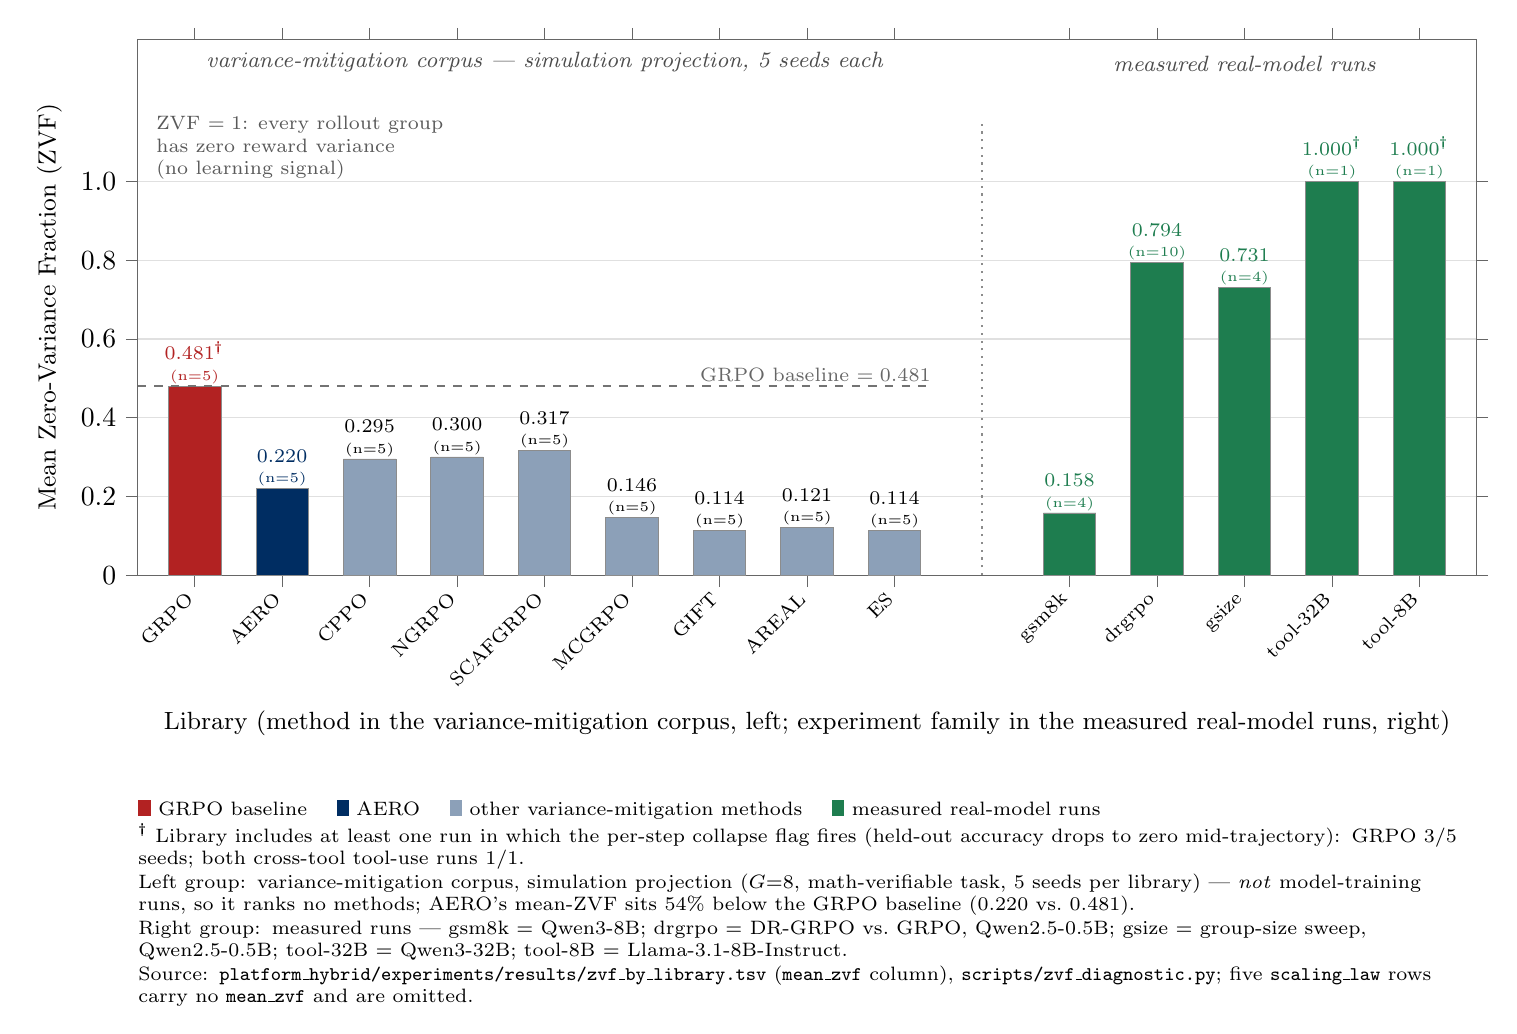
\begin{tikzpicture}
\begin{axis}[
    width=17cm, height=6.8cm,
    scale only axis,
    xmin=-0.65, xmax=14.65,
    ymin=0, ymax=1.36,
    ytick={0,0.2,0.4,0.6,0.8,1.0},
    yticklabels={0,0.2,0.4,0.6,0.8,1.0},
    ylabel={Mean Zero-Variance Fraction (ZVF)},
    ylabel style={font=\small},
    xlabel={Library (method in the variance-mitigation corpus, left; experiment family in the measured real-model runs, right)},
    xlabel style={font=\small},
    xtick={0,1,2,3,4,5,6,7,8,10,11,12,13,14},
    xticklabels={GRPO,AERO,CPPO,NGRPO,SCAFGRPO,MCGRPO,GIFT,AREAL,ES,%
                 gsm8k,drgrpo,gsize,tool-32B,tool-8B},
    xticklabel style={rotate=45, anchor=east, font=\scriptsize, yshift=-1pt},
    tick align=outside,
    ymajorgrids=true,
    grid style={draw=black!12},
    axis line style={draw=black!60},
    tick style={draw=black!60},
    every axis plot/.append style={ybar, bar shift=0pt, bar width=0.60},
    clip=false,
]

% ---- bars: colour groups the corpus, but each bar is named on the x axis ----
% variance-mitigation methods other than GRPO/AERO
\addplot[fill=pesblue!45, draw=black!45, line width=0.25pt] coordinates {
  (2,0.2952) (3,0.3003) (4,0.3166) (5,0.1461) (6,0.1142) (7,0.1209) (8,0.1142)};
% AERO (method the diagnostic is read against)
\addplot[fill=pesblue, draw=black!45, line width=0.25pt] coordinates {(1,0.2203)};
% GRPO baseline
\addplot[fill=bad, draw=black!45, line width=0.25pt] coordinates {(0,0.4808)};
% measured real-model runs
\addplot[fill=complete, draw=black!45, line width=0.25pt] coordinates {
  (10,0.1583) (11,0.7941) (12,0.7308) (13,1.0000) (14,1.0000)};

% ---- GRPO baseline reference line over the mitigation corpus ----
\draw[dashed, black!55, thick] (axis cs:-0.65,0.4808) -- (axis cs:8.45,0.4808);
\node[anchor=south east, font=\scriptsize, text=black!60, inner sep=1pt]
  at (axis cs:8.45,0.4840) {GRPO baseline $=0.481$};

% ---- corpus divider ----
\draw[dotted, black!45, thick] (axis cs:9.0,0) -- (axis cs:9.0,1.16);

% ---- per-bar value and run-count labels (bar top + small offset) ----
% mitigation corpus: 5 seeds / 5 rows per library
\node[anchor=south, align=center, font=\scriptsize, inner sep=0.6pt, text=bad]
  at (axis cs:0,0.4808) {0.481\textsuperscript{\dag}\\[-0.2ex]{\tiny (n=5)}};
\node[anchor=south, align=center, font=\scriptsize, inner sep=0.6pt, text=pesblue]
  at (axis cs:1,0.2203) {0.220\\[-0.2ex]{\tiny (n=5)}};
\node[anchor=south, align=center, font=\scriptsize, inner sep=0.6pt]
  at (axis cs:2,0.2952) {0.295\\[-0.2ex]{\tiny (n=5)}};
\node[anchor=south, align=center, font=\scriptsize, inner sep=0.6pt]
  at (axis cs:3,0.3003) {0.300\\[-0.2ex]{\tiny (n=5)}};
\node[anchor=south, align=center, font=\scriptsize, inner sep=0.6pt]
  at (axis cs:4,0.3166) {0.317\\[-0.2ex]{\tiny (n=5)}};
\node[anchor=south, align=center, font=\scriptsize, inner sep=0.6pt]
  at (axis cs:5,0.1461) {0.146\\[-0.2ex]{\tiny (n=5)}};
\node[anchor=south, align=center, font=\scriptsize, inner sep=0.6pt]
  at (axis cs:6,0.1142) {0.114\\[-0.2ex]{\tiny (n=5)}};
\node[anchor=south, align=center, font=\scriptsize, inner sep=0.6pt]
  at (axis cs:7,0.1209) {0.121\\[-0.2ex]{\tiny (n=5)}};
\node[anchor=south, align=center, font=\scriptsize, inner sep=0.6pt]
  at (axis cs:8,0.1142) {0.114\\[-0.2ex]{\tiny (n=5)}};
% measured real-model runs: rows behind each bar
\node[anchor=south, align=center, font=\scriptsize, inner sep=0.6pt, text=complete]
  at (axis cs:10,0.1583) {0.158\\[-0.2ex]{\tiny (n=4)}};
\node[anchor=south, align=center, font=\scriptsize, inner sep=0.6pt, text=complete]
  at (axis cs:11,0.7941) {0.794\\[-0.2ex]{\tiny (n=10)}};
\node[anchor=south, align=center, font=\scriptsize, inner sep=0.6pt, text=complete]
  at (axis cs:12,0.7308) {0.731\\[-0.2ex]{\tiny (n=4)}};
\node[anchor=south, align=center, font=\scriptsize, inner sep=0.6pt, text=complete]
  at (axis cs:13,1.0000) {1.000\textsuperscript{\dag}\\[-0.2ex]{\tiny (n=1)}};
\node[anchor=south, align=center, font=\scriptsize, inner sep=0.6pt, text=complete]
  at (axis cs:14,1.0000) {1.000\textsuperscript{\dag}\\[-0.2ex]{\tiny (n=1)}};

% ---- corpus group labels ----
\node[anchor=south, font=\footnotesize\itshape, text=black!70]
  at (axis cs:4.0,1.255) {variance-mitigation corpus --- simulation projection, 5 seeds each};
\node[anchor=south, font=\footnotesize\itshape, text=black!70]
  at (axis cs:12.0,1.255) {measured real-model runs};

% ---- definitional note in the free upper-left region ----
\node[anchor=north west, align=left, font=\scriptsize, text=black!65]
  at (axis cs:-0.55,1.19) {ZVF $=1$: every rollout group\\ has zero reward variance\\(no learning signal)};

\end{axis}

% ---- footer: colour key, marker key, corpus boundary, provenance ----
\node[anchor=north west, align=left, text width=16.8cm, font=\scriptsize, inner sep=0pt]
  at ($(current axis.south west)+(0cm,-2.85cm)$) {%
  \textcolor{bad}{\rule{1.6mm}{2.0mm}}~GRPO baseline \quad
  \textcolor{pesblue}{\rule{1.6mm}{2.0mm}}~AERO \quad
  \textcolor{pesblue!45}{\rule{1.6mm}{2.0mm}}~other variance-mitigation methods \quad
  \textcolor{complete}{\rule{1.6mm}{2.0mm}}~measured real-model runs
  \\[0.5ex]
  \textsuperscript{\dag}~Library includes at least one run in which the per-step collapse flag fires (held-out accuracy drops to zero mid-trajectory): GRPO 3/5 seeds; both cross-tool tool-use runs 1/1.
  \\[0.2ex]
  Left group: variance-mitigation corpus, simulation projection ($G{=}8$, math-verifiable task, 5 seeds per library) --- \emph{not} model-training runs, so it ranks no methods; AERO's mean-ZVF sits $54\%$ below the GRPO baseline ($0.220$ vs.\ $0.481$).
  \\[0.2ex]
  Right group: measured runs --- gsm8k $=$ Qwen3-8B; drgrpo $=$ DR-GRPO vs.\ GRPO, Qwen2.5-0.5B; gsize $=$ group-size sweep, Qwen2.5-0.5B; tool-32B $=$ Qwen3-32B; tool-8B $=$ Llama-3.1-8B-Instruct.
  \\[0.2ex]
  Source: \texttt{platform\_hybrid/experiments/results/zvf\_by\_library.tsv} (\texttt{mean\_zvf} column), \texttt{scripts/zvf\_diagnostic.py}; five \texttt{scaling\_law} rows carry no \texttt{mean\_zvf} and are omitted.};
\end{tikzpicture}
\end{document}
